% Options for packages loaded elsewhere
\PassOptionsToPackage{unicode}{hyperref}
\PassOptionsToPackage{hyphens}{url}
\PassOptionsToPackage{dvipsnames,svgnames,x11names}{xcolor}
%
\documentclass[
  letterpaper,
  DIV=11,
  numbers=noendperiod]{scrartcl}

\usepackage{amsmath,amssymb}
\usepackage{iftex}
\ifPDFTeX
  \usepackage[T1]{fontenc}
  \usepackage[utf8]{inputenc}
  \usepackage{textcomp} % provide euro and other symbols
\else % if luatex or xetex
  \usepackage{unicode-math}
  \defaultfontfeatures{Scale=MatchLowercase}
  \defaultfontfeatures[\rmfamily]{Ligatures=TeX,Scale=1}
\fi
\usepackage{lmodern}
\ifPDFTeX\else  
    % xetex/luatex font selection
\fi
% Use upquote if available, for straight quotes in verbatim environments
\IfFileExists{upquote.sty}{\usepackage{upquote}}{}
\IfFileExists{microtype.sty}{% use microtype if available
  \usepackage[]{microtype}
  \UseMicrotypeSet[protrusion]{basicmath} % disable protrusion for tt fonts
}{}
\makeatletter
\@ifundefined{KOMAClassName}{% if non-KOMA class
  \IfFileExists{parskip.sty}{%
    \usepackage{parskip}
  }{% else
    \setlength{\parindent}{0pt}
    \setlength{\parskip}{6pt plus 2pt minus 1pt}}
}{% if KOMA class
  \KOMAoptions{parskip=half}}
\makeatother
\usepackage{xcolor}
\setlength{\emergencystretch}{3em} % prevent overfull lines
\setcounter{secnumdepth}{-\maxdimen} % remove section numbering
% Make \paragraph and \subparagraph free-standing
\ifx\paragraph\undefined\else
  \let\oldparagraph\paragraph
  \renewcommand{\paragraph}[1]{\oldparagraph{#1}\mbox{}}
\fi
\ifx\subparagraph\undefined\else
  \let\oldsubparagraph\subparagraph
  \renewcommand{\subparagraph}[1]{\oldsubparagraph{#1}\mbox{}}
\fi

\usepackage{color}
\usepackage{fancyvrb}
\newcommand{\VerbBar}{|}
\newcommand{\VERB}{\Verb[commandchars=\\\{\}]}
\DefineVerbatimEnvironment{Highlighting}{Verbatim}{commandchars=\\\{\}}
% Add ',fontsize=\small' for more characters per line
\usepackage{framed}
\definecolor{shadecolor}{RGB}{241,243,245}
\newenvironment{Shaded}{\begin{snugshade}}{\end{snugshade}}
\newcommand{\AlertTok}[1]{\textcolor[rgb]{0.68,0.00,0.00}{#1}}
\newcommand{\AnnotationTok}[1]{\textcolor[rgb]{0.37,0.37,0.37}{#1}}
\newcommand{\AttributeTok}[1]{\textcolor[rgb]{0.40,0.45,0.13}{#1}}
\newcommand{\BaseNTok}[1]{\textcolor[rgb]{0.68,0.00,0.00}{#1}}
\newcommand{\BuiltInTok}[1]{\textcolor[rgb]{0.00,0.23,0.31}{#1}}
\newcommand{\CharTok}[1]{\textcolor[rgb]{0.13,0.47,0.30}{#1}}
\newcommand{\CommentTok}[1]{\textcolor[rgb]{0.37,0.37,0.37}{#1}}
\newcommand{\CommentVarTok}[1]{\textcolor[rgb]{0.37,0.37,0.37}{\textit{#1}}}
\newcommand{\ConstantTok}[1]{\textcolor[rgb]{0.56,0.35,0.01}{#1}}
\newcommand{\ControlFlowTok}[1]{\textcolor[rgb]{0.00,0.23,0.31}{#1}}
\newcommand{\DataTypeTok}[1]{\textcolor[rgb]{0.68,0.00,0.00}{#1}}
\newcommand{\DecValTok}[1]{\textcolor[rgb]{0.68,0.00,0.00}{#1}}
\newcommand{\DocumentationTok}[1]{\textcolor[rgb]{0.37,0.37,0.37}{\textit{#1}}}
\newcommand{\ErrorTok}[1]{\textcolor[rgb]{0.68,0.00,0.00}{#1}}
\newcommand{\ExtensionTok}[1]{\textcolor[rgb]{0.00,0.23,0.31}{#1}}
\newcommand{\FloatTok}[1]{\textcolor[rgb]{0.68,0.00,0.00}{#1}}
\newcommand{\FunctionTok}[1]{\textcolor[rgb]{0.28,0.35,0.67}{#1}}
\newcommand{\ImportTok}[1]{\textcolor[rgb]{0.00,0.46,0.62}{#1}}
\newcommand{\InformationTok}[1]{\textcolor[rgb]{0.37,0.37,0.37}{#1}}
\newcommand{\KeywordTok}[1]{\textcolor[rgb]{0.00,0.23,0.31}{#1}}
\newcommand{\NormalTok}[1]{\textcolor[rgb]{0.00,0.23,0.31}{#1}}
\newcommand{\OperatorTok}[1]{\textcolor[rgb]{0.37,0.37,0.37}{#1}}
\newcommand{\OtherTok}[1]{\textcolor[rgb]{0.00,0.23,0.31}{#1}}
\newcommand{\PreprocessorTok}[1]{\textcolor[rgb]{0.68,0.00,0.00}{#1}}
\newcommand{\RegionMarkerTok}[1]{\textcolor[rgb]{0.00,0.23,0.31}{#1}}
\newcommand{\SpecialCharTok}[1]{\textcolor[rgb]{0.37,0.37,0.37}{#1}}
\newcommand{\SpecialStringTok}[1]{\textcolor[rgb]{0.13,0.47,0.30}{#1}}
\newcommand{\StringTok}[1]{\textcolor[rgb]{0.13,0.47,0.30}{#1}}
\newcommand{\VariableTok}[1]{\textcolor[rgb]{0.07,0.07,0.07}{#1}}
\newcommand{\VerbatimStringTok}[1]{\textcolor[rgb]{0.13,0.47,0.30}{#1}}
\newcommand{\WarningTok}[1]{\textcolor[rgb]{0.37,0.37,0.37}{\textit{#1}}}

\providecommand{\tightlist}{%
  \setlength{\itemsep}{0pt}\setlength{\parskip}{0pt}}\usepackage{longtable,booktabs,array}
\usepackage{calc} % for calculating minipage widths
% Correct order of tables after \paragraph or \subparagraph
\usepackage{etoolbox}
\makeatletter
\patchcmd\longtable{\par}{\if@noskipsec\mbox{}\fi\par}{}{}
\makeatother
% Allow footnotes in longtable head/foot
\IfFileExists{footnotehyper.sty}{\usepackage{footnotehyper}}{\usepackage{footnote}}
\makesavenoteenv{longtable}
\usepackage{graphicx}
\makeatletter
\def\maxwidth{\ifdim\Gin@nat@width>\linewidth\linewidth\else\Gin@nat@width\fi}
\def\maxheight{\ifdim\Gin@nat@height>\textheight\textheight\else\Gin@nat@height\fi}
\makeatother
% Scale images if necessary, so that they will not overflow the page
% margins by default, and it is still possible to overwrite the defaults
% using explicit options in \includegraphics[width, height, ...]{}
\setkeys{Gin}{width=\maxwidth,height=\maxheight,keepaspectratio}
% Set default figure placement to htbp
\makeatletter
\def\fps@figure{htbp}
\makeatother

\KOMAoption{captions}{tableheading}
\makeatletter
\@ifpackageloaded{tcolorbox}{}{\usepackage[skins,breakable]{tcolorbox}}
\@ifpackageloaded{fontawesome5}{}{\usepackage{fontawesome5}}
\definecolor{quarto-callout-color}{HTML}{909090}
\definecolor{quarto-callout-note-color}{HTML}{0758E5}
\definecolor{quarto-callout-important-color}{HTML}{CC1914}
\definecolor{quarto-callout-warning-color}{HTML}{EB9113}
\definecolor{quarto-callout-tip-color}{HTML}{00A047}
\definecolor{quarto-callout-caution-color}{HTML}{FC5300}
\definecolor{quarto-callout-color-frame}{HTML}{acacac}
\definecolor{quarto-callout-note-color-frame}{HTML}{4582ec}
\definecolor{quarto-callout-important-color-frame}{HTML}{d9534f}
\definecolor{quarto-callout-warning-color-frame}{HTML}{f0ad4e}
\definecolor{quarto-callout-tip-color-frame}{HTML}{02b875}
\definecolor{quarto-callout-caution-color-frame}{HTML}{fd7e14}
\makeatother
\makeatletter
\@ifpackageloaded{caption}{}{\usepackage{caption}}
\AtBeginDocument{%
\ifdefined\contentsname
  \renewcommand*\contentsname{Table of contents}
\else
  \newcommand\contentsname{Table of contents}
\fi
\ifdefined\listfigurename
  \renewcommand*\listfigurename{List of Figures}
\else
  \newcommand\listfigurename{List of Figures}
\fi
\ifdefined\listtablename
  \renewcommand*\listtablename{List of Tables}
\else
  \newcommand\listtablename{List of Tables}
\fi
\ifdefined\figurename
  \renewcommand*\figurename{Figure}
\else
  \newcommand\figurename{Figure}
\fi
\ifdefined\tablename
  \renewcommand*\tablename{Table}
\else
  \newcommand\tablename{Table}
\fi
}
\@ifpackageloaded{float}{}{\usepackage{float}}
\floatstyle{ruled}
\@ifundefined{c@chapter}{\newfloat{codelisting}{h}{lop}}{\newfloat{codelisting}{h}{lop}[chapter]}
\floatname{codelisting}{Listing}
\newcommand*\listoflistings{\listof{codelisting}{List of Listings}}
\makeatother
\makeatletter
\makeatother
\makeatletter
\@ifpackageloaded{caption}{}{\usepackage{caption}}
\@ifpackageloaded{subcaption}{}{\usepackage{subcaption}}
\makeatother
\ifLuaTeX
  \usepackage{selnolig}  % disable illegal ligatures
\fi
\usepackage{bookmark}

\IfFileExists{xurl.sty}{\usepackage{xurl}}{} % add URL line breaks if available
\urlstyle{same} % disable monospaced font for URLs
\hypersetup{
  pdftitle={Python},
  pdfauthor={Pablo Winant},
  colorlinks=true,
  linkcolor={blue},
  filecolor={Maroon},
  citecolor={Blue},
  urlcolor={Blue},
  pdfcreator={LaTeX via pandoc}}

\title{Python}
\usepackage{etoolbox}
\makeatletter
\providecommand{\subtitle}[1]{% add subtitle to \maketitle
  \apptocmd{\@title}{\par {\large #1 \par}}{}{}
}
\makeatother
\subtitle{Computational Economics @ Bundesbank}
\author{Pablo Winant}
\date{}

\begin{document}
\maketitle

\section{Why Python???}\label{why-python}

. . .

\begin{figure}[H]

{\centering 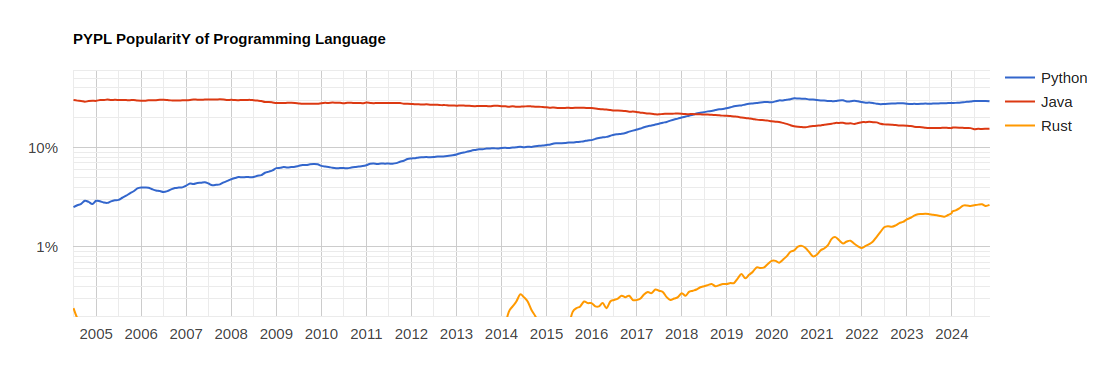
\includegraphics{graphs/popularity.png}

}

\caption{Center}

\end{figure}%

. . .

Python:

\begin{itemize}
\tightlist
\item
  is popular
\item
  is free and opensource
\item
  has many many libraries
\item
  vibrant community
\item
  lots of online resources
\end{itemize}

\subsection{Dummy slide}\label{dummy-slide}

\begin{Shaded}
\begin{Highlighting}[]
\ImportTok{import}\NormalTok{ numpy }\ImportTok{as}\NormalTok{ np}
\ImportTok{from}\NormalTok{ matplotlib }\ImportTok{import}\NormalTok{ pyplot }\ImportTok{as}\NormalTok{ plt}
\NormalTok{x }\OperatorTok{=}\NormalTok{ np.linspace(}\DecValTok{0}\NormalTok{,}\DecValTok{1}\NormalTok{,}\DecValTok{100}\NormalTok{)}
\NormalTok{y }\OperatorTok{=}\NormalTok{ x}\OperatorTok{**}\DecValTok{2}
\NormalTok{plt.plot(x,y)}
\end{Highlighting}
\end{Shaded}

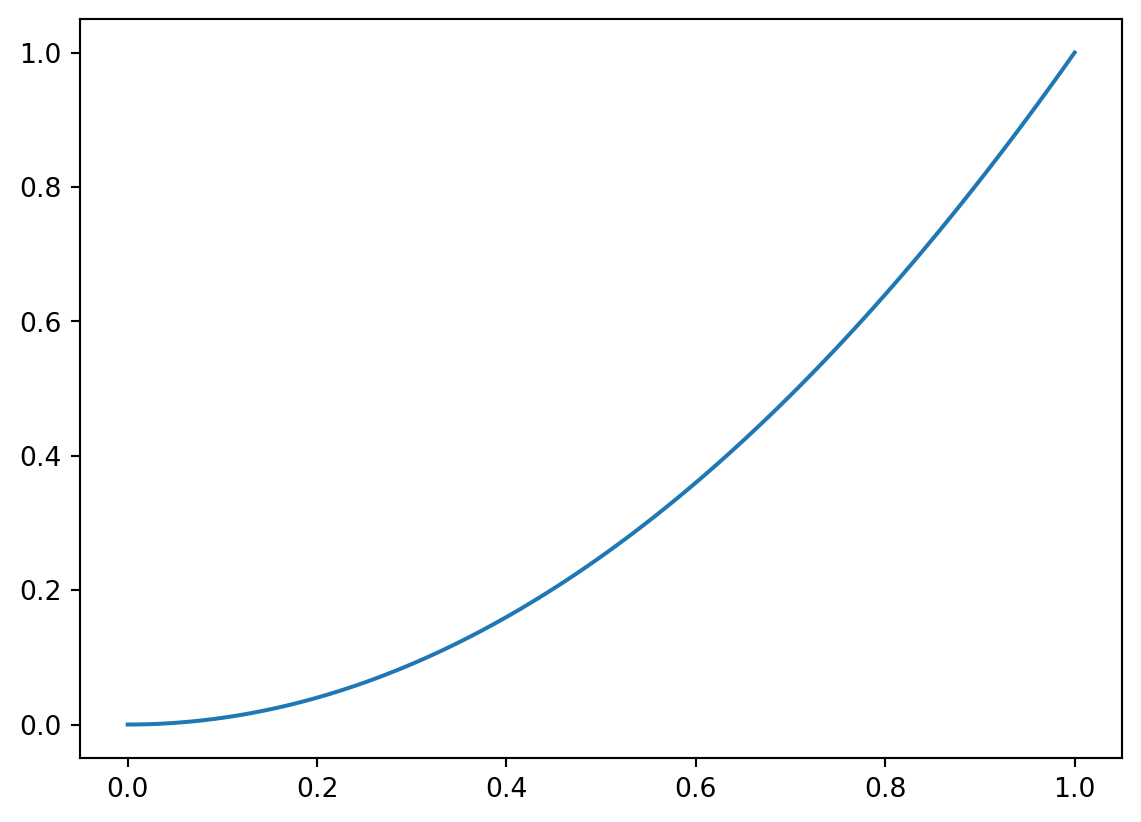
\includegraphics{python_files/figure-latex/cell-2-output-1.pdf}

\subsection{Why Python? (3)}\label{why-python-3}

Historically, python was a glue language used to interoperate many
low-level/system languages.

It has been increasingly used for web-development (cf django)

. . .

Nowadays it is the lingua franca of machine learning

Most major machine learning / deep learning libraries have python
bindings

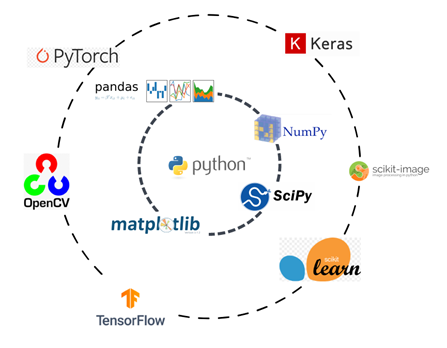
\includegraphics{graphs/python_ml.png}

\subsection{An example}\label{an-example}

\begin{Shaded}
\begin{Highlighting}[]
\KeywordTok{def}\NormalTok{ say\_hello(name):}
    \CommentTok{"""This function prints morning greetings"""}

    \BuiltInTok{print}\NormalTok{(}\SpecialStringTok{f"Good morning }\SpecialCharTok{\{}\NormalTok{name}\SpecialCharTok{\}}\SpecialStringTok{!}\CharTok{\textbackslash{}n}\SpecialStringTok{"}\NormalTok{)}

    \CommentTok{\# we can import libraries}
    \ImportTok{import}\NormalTok{ datetime}
\NormalTok{    t }\OperatorTok{=}\NormalTok{ datetime.datetime.now()}

    \CommentTok{\# blocks are defined by indentation and colons}
    \ControlFlowTok{if}\NormalTok{ (t.hour,t.}\BuiltInTok{min}\NormalTok{) }\OperatorTok{\textless{}=}\NormalTok{ (}\DecValTok{9}\NormalTok{,}\DecValTok{15}\NormalTok{):}
        \BuiltInTok{print}\NormalTok{(}\StringTok{"All good?}\CharTok{\textbackslash{}n}\StringTok{"}\NormalTok{)}
    \ControlFlowTok{else}\NormalTok{:}
        \BuiltInTok{print}\NormalTok{(}\StringTok{"Time to get started?}\CharTok{\textbackslash{}n}\StringTok{"}\NormalTok{)}


\NormalTok{say\_hello(}\StringTok{"Pablo"}\NormalTok{)}
\end{Highlighting}
\end{Shaded}

\subsection{Python is everywhere}\label{python-is-everywhere}

\begin{figure}[H]

{\centering 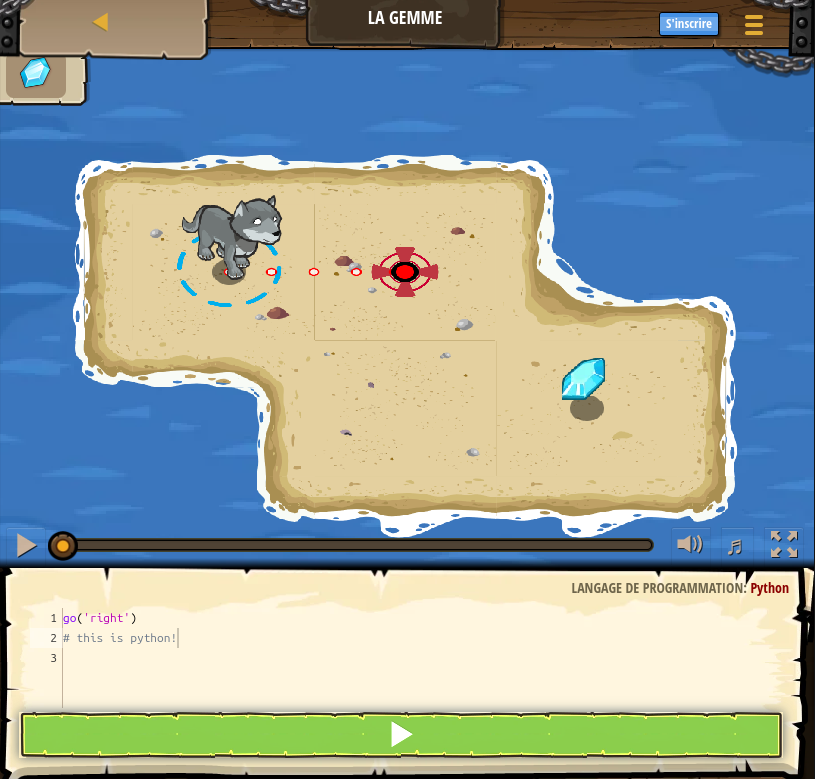
\includegraphics{graphs/code_warrior.png}

}

\caption{Code Warriors}

\end{figure}%

\begin{figure}[H]

{\centering \includegraphics{graphs/microbits.webp}

}

\caption{MicroBits}

\end{figure}%

\begin{itemize}
\item
  Windows
\item
  Linux
\item
  Web
\end{itemize}

\subsection{The Python family}\label{the-python-family}

There are several flavours of Python:

\begin{itemize}
\tightlist
\item
  Full Syntax

  \begin{itemize}
  \tightlist
  \item
    CPython, PyPy, Pyston
  \end{itemize}
\item
  Subset-Syntax

  \begin{itemize}
  \tightlist
  \item
    micropython
  \item
    numba, pythran
  \end{itemize}
\end{itemize}

\begin{itemize}
\tightlist
\item
  Superset-Syntax

  \begin{itemize}
  \tightlist
  \item
    mypy (*)
  \item
    cython
  \item
    mojo
  \end{itemize}
\item
  Near-Syntax

  \begin{itemize}
  \tightlist
  \item
    boo
  \end{itemize}
\end{itemize}

\begin{itemize}
\tightlist
\item
  subset-syntax: restrict functionalities (no classes, simpler objects)
  for easier compilation
\item
  superset-syntax: add type/memory information
\item
  near-syntax: different language that looks familiar
\end{itemize}

\subsection{Examples}\label{examples}

\begin{itemize}
\tightlist
\item
  mojo:
\end{itemize}

\begin{Shaded}
\begin{Highlighting}[]
\NormalTok{fn greet2(name: String) {-}\textgreater{} String:}
\NormalTok{    return "Hello, " + name + "!"}
\end{Highlighting}
\end{Shaded}

\begin{itemize}
\tightlist
\item
  cython
\end{itemize}

\begin{Shaded}
\begin{Highlighting}[]
\NormalTok{from libcpp.vector cimport vector}

\NormalTok{def primes(unsigned int nb\_primes):}

\NormalTok{    cdef int n, i}
\NormalTok{    cdef vector[int] p}
\NormalTok{    p.reserve(nb\_primes)  \# allocate memory for \textquotesingle{}nb\_primes\textquotesingle{} elements.}

\NormalTok{    n = 2}
\NormalTok{    while p.size() \textless{} nb\_primes:  \# size() for vectors is similar to len()}
\NormalTok{        for i in p:}
\NormalTok{            if n \% i == 0:}
\NormalTok{                break }
\end{Highlighting}
\end{Shaded}

\subsection{Python is interpreted}\label{python-is-interpreted}

\begin{tcolorbox}[enhanced jigsaw, opacityback=0, breakable, bottomrule=.15mm, bottomtitle=1mm, opacitybacktitle=0.6, left=2mm, coltitle=black, titlerule=0mm, leftrule=.75mm, toprule=.15mm, colback=white, toptitle=1mm, title=\textcolor{quarto-callout-note-color}{\faInfo}\hspace{0.5em}{Interpreted language}, arc=.35mm, rightrule=.15mm, colframe=quarto-callout-note-color-frame, colbacktitle=quarto-callout-note-color!10!white]

In an interpreted language, instructions are read and translated into
processor instructions, one after another.

\end{tcolorbox}

As consequence, it is:

\begin{itemize}
\tightlist
\item
  flexible

  \begin{itemize}
  \tightlist
  \item
    interactive development
  \item
    immediate feedback
  \end{itemize}
\item
  slooooww \footnote{actualy not so much because python modules are
    converted into bytecode and because common objects are well
    optimized}
\end{itemize}

\subsection{Intepreters}\label{intepreters}

\begin{itemize}
\tightlist
\item
  Python
\item
  ipython a.k.a. jupyter

  \begin{itemize}
  \tightlist
  \item
    send instructions to a kernel
  \item
    receive back MIME objects (with nice html representation)
  \end{itemize}
\item
  VSCode

  \begin{itemize}
  \tightlist
  \item
    has its own python kernel implementation
  \end{itemize}
\item
  C API python.h

  \begin{itemize}
  \tightlist
  \item
    julia
  \item
    your own\ldots{}
  \end{itemize}
\end{itemize}

\section{Packages and Environment}\label{packages-and-environment}

\subsection{Python modules}\label{python-modules}

A file ending with .py is a \emph{python module}

\begin{itemize}
\tightlist
\item
  \texttt{program.py}
\end{itemize}

\begin{Shaded}
\begin{Highlighting}[]
\NormalTok{key }\OperatorTok{=} \StringTok{"low"}
\KeywordTok{def}\NormalTok{ something():}
    \ControlFlowTok{return} \StringTok{"hey"}
\end{Highlighting}
\end{Shaded}

The content from a module can be \emph{imported}

\begin{Shaded}
\begin{Highlighting}[]
\ImportTok{from}\NormalTok{ program }\ImportTok{import}\NormalTok{ something}
\end{Highlighting}
\end{Shaded}

To import all objects in a module (functions, strings, \ldots)

\begin{Shaded}
\begin{Highlighting}[]
\ImportTok{from}\NormalTok{ program }\ImportTok{import} \OperatorTok{*}
\end{Highlighting}
\end{Shaded}

\subsection{Submodules}\label{submodules}

\begin{itemize}
\item
  A folder containing modules and an \texttt{\_\_init.py\_\_} is a
  \texttt{package}.
\item
  import a package or a submodule:

  \begin{itemize}
  \tightlist
  \item
    \texttt{import\ package}
  \item
    \texttt{from\ package.submodule\ import\ something}
  \end{itemize}
\item
  The content of modules and submodules is evaluated only
  once.\footnote{since python 3.4 you can actually reload a module with
    \texttt{importlib.reload()}}
\item
  It is actually precompiled.
\item
  This is perfect for distributing a package.
\item
  Not so much to develop code interactively.
\end{itemize}

\subsection{Package managers}\label{package-managers}

Several ways to create / distribute python packages have been developped
over the years.

\begin{itemize}
\tightlist
\item
  setup.py, pip
\item
  setuptools, distutils, \ldots{}
\item
  pipenv, poetry, \ldots{}
\item
  conda
\end{itemize}

There are essentially two kinds of packages:

\begin{itemize}
\tightlist
\item
  pip packages
\item
  conda packages
\end{itemize}

\subsection{Pip packages}\label{pip-packages}

\begin{itemize}
\item
  pip files (what are eggs btw)

  \begin{itemize}
  \tightlist
  \item
    pure python
  \item
    binary
  \end{itemize}
\item
  can be installed with \texttt{pip\ install\ package}
\item
  no dependency solving ! no proper uninstallation !
\item
  pip files a virtual evnironment created with \texttt{venv}
\item
  reproducible setup can be described in

  \begin{itemize}
  \tightlist
  \item
    requirements.txt (old)
  \item
    pyproject.toml (new)
  \end{itemize}
\item
  directory specific environments can be managed with \texttt{poetry} or
  \texttt{venv}:

  \begin{itemize}
  \tightlist
  \item
    \texttt{python\ -m\ venv\ directory}
  \end{itemize}
\end{itemize}

\subsection{Conda environment}\label{conda-environment}

\begin{itemize}
\item
  conda files
\item
  installed in a conda environment
\item
  with proper / reversible dependency solving

  \begin{itemize}
  \tightlist
  \item
    very quick using \texttt{mamba} or \texttt{micromamba}
  \end{itemize}
\item
  reproducible environment can be described in:

  \begin{itemize}
  \tightlist
  \item
    environment.yml (dependencies)
  \item
    manifest (\ldots)
  \end{itemize}
\item
  directory specific environments can be managed with \texttt{pixi}
\end{itemize}

\section{Syntax Review}\label{syntax-review}

\subsection{}\label{section}

Let's setup the environment specified in
\href{../requirements.txt}{requirements.txt}

. . .


\includegraphics{graphs/ea0.jpg}

Move to \href{../handson/python_syntax.qmd}{python syntax} tutorial



\end{document}
